\documentclass[fontsize=10pt,twoside=false]{kaobook}
\usepackage[english]{babel}
\usepackage{tikz}
\usetikzlibrary{arrows.meta, positioning, calc, shapes.geometric, shapes.misc, fit, backgrounds}

\begin{document}
\mainmatter
\chapter{probe}
\begin{figure}[h]
	\centering
	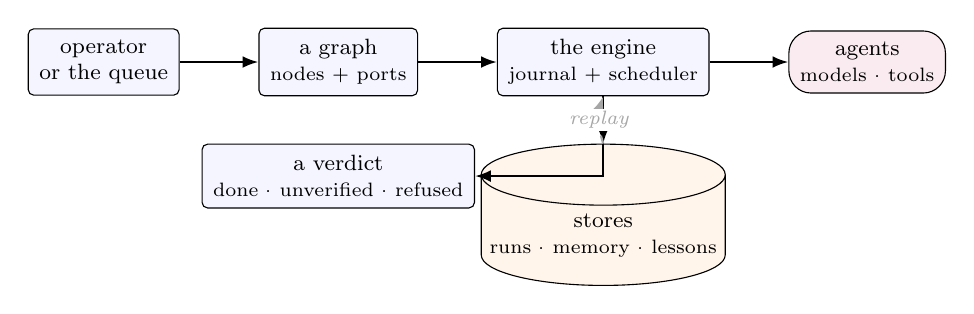
\begin{tikzpicture}[node distance=6mm and 10mm]
		\node[draw, rounded corners=2pt, fill=blue!4, align=center, inner sep=4pt, font=\footnotesize] (user) {operator\\or the queue};
		\node[draw, rounded corners=2pt, fill=blue!4, align=center, inner sep=4pt, font=\footnotesize, right=of user] (graph) {a graph\\\scriptsize nodes + ports};
		\node[draw, rounded corners=2pt, fill=blue!4, align=center, inner sep=4pt, font=\footnotesize, right=of graph] (engine) {the engine\\\scriptsize journal + scheduler};
		\node[draw, cylinder, shape border rotate=90, aspect=0.25, fill=orange!8, align=center, inner sep=3pt, font=\footnotesize, below=of engine] (stores) {stores\\\scriptsize runs · memory · lessons};
		\node[draw, rounded corners=8pt, fill=purple!8, align=center, inner sep=4pt, font=\footnotesize, right=of engine] (agents) {agents\\\scriptsize models · tools};
		\node[draw, rounded corners=2pt, fill=blue!4, align=center, inner sep=4pt, font=\footnotesize, below=of graph] (verdict) {a verdict\\\scriptsize done · unverified · refused};

		\draw[-{Latex[length=2mm]}, thick] (user) -- (graph);
		\draw[-{Latex[length=2mm]}, thick] (graph) -- (engine);
		\draw[-{Latex[length=2mm]}, thick] (engine) -- (stores);
		\draw[-{Latex[length=2mm]}, thick] (engine) -- (agents);
		\draw[-{Latex[length=2mm]}, thick] (engine) |- (verdict);
		\draw[-{Latex[length=2mm]}, thick, dashed, gray!70] (stores.north) to[bend left=18] node[font=\scriptsize\itshape, inner sep=1pt, fill=white]{replay} (engine.south);
	\end{tikzpicture}
	\caption{A run's shape. The arrow that matters is the dashed one: the stores can reconstruct
	what the engine did, which is what makes a verdict checkable rather than asserted.}
\end{figure}
\end{document}
